%\renewcommand{\theequation}{\theenumi}
%\begin{enumerate}[label=\arabic*.,ref=\theenumi]
\begin{enumerate}[label=\thesection.\arabic*.,ref=\thesection.\theenumi]
\numberwithin{equation}{enumi}
\item If $\vec{D}$ divides $BC$ in the ratio $k : 1$,
		\begin{align}
			\vec{D}= \frac{k\vec{C}+\vec{B}}{k+1}
		\end{align}
		Find the mid points $\vec{D}, \vec{E}, \vec{F}$ of the sides $BC, CA$ and $AB$ respectively.
	\\
		\solution
Since $\vec{D}$ is the midpoint of $BC$,
\begin{align}
k &= 1,\\
\implies \vec{D} &= \frac{\vec{C} + \vec{B}}{2}
= \frac{1}{2}\myvec{-7\\1}
\end{align}
Similarly,
\begin{align}
\vec{E} &= \frac{\vec{A} + \vec{C}}{2}
= \myvec{-1\\-3}\\
\vec{F} &= \frac{\vec{A} + \vec{B}}{2}
= \frac{1}{2}\myvec{-3\\5}
\end{align}
  
	\item Find the equations of $AD, BE$ and $CF$.
	\\	\\ \solution:
\begin{enumerate}
 \item The direction vector of $AD$ is 
\begin{align}
	\vec{m} = \vec{D}- \vec{A}
&=\myvec{\frac{-7}{2}\\\frac{1}{2}} - \myvec{1\\-1}
	=\frac{1}{2}\myvec{-9\\3} \equiv \myvec{-3 \\ 1}
	\\
	\implies  \vec{n} &=\myvec{1 \\ 3}
\end{align}
Hence the normal equation of median $AD$ is 
\begin{align}
\vec{n}^{\top}\myvec{\vec{x}-\vec{A}}&=0\\
\implies    \myvec{1 & 3}\vec{x}&=\myvec{1 & 3}\myvec{1\\-1}
    =-2
	\label{eq:median-ad}
\end{align}
\item For $BE$,
\begin{align}
	\vec{m}= \vec{E}- \vec{B}&=\myvec{-1\\-3} - \myvec{-4\\6}
       =\myvec{3\\-9}
       \equiv \myvec{1\\-3}
       \\
\implies 	
\vec{n} &= 
         \myvec{3\\1}
\end{align}
Hence the normal equation of median $BE$ is 
\begin{align}
\vec{n}^{\top}\myvec{\vec{x}-\vec{B}}&=0\\
\implies
	\myvec{3 & 1}   \vec{x}&=\myvec{3 &1}\myvec{-4\\6}
    =-6
	\label{eq:median-be}
\end{align}
\item For median $CF$,
\begin{align}
	\vec{m} = \vec{F}- \vec{C} &=
\myvec{\frac{-3}{2}\\\frac{5}{2}} - \myvec{-3\\-5}
       =\myvec{\frac{3}{2}\\\frac{15}{2}}
       \equiv \myvec{1 \\ 5}
       \\
	\implies \vec{n} &=\myvec{5 \\ -1}
\end{align}
Hence the normal equation of median $CF$ is 
\begin{align}
\vec{n}^{\top}\myvec{\vec{x}-\vec{C}}&=0\\
	\implies \myvec{5 & -1}\vec{x}&=\myvec{5 & -1}\myvec{-3\\-5}
    =-10
	\label{eq:median-cf}
\end{align}
\end{enumerate}
\iffalse
\begin{figure}
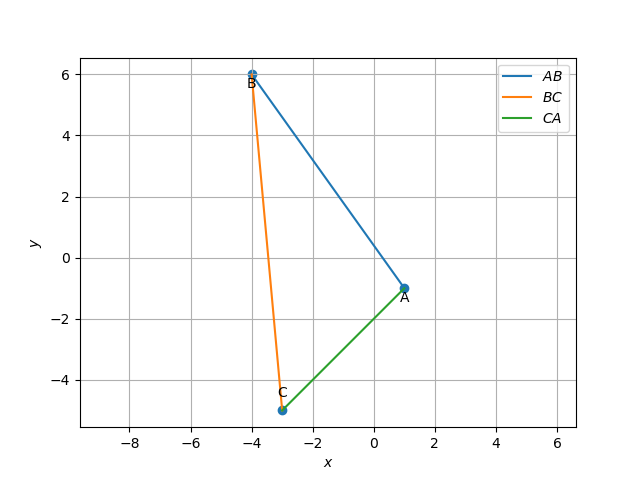
\includegraphics [width=\columnwidth] {solutions/1/2/2/figs/figure.png}
\caption{ Medians $AD$ , $BE$ and $CF$}
\label{fig: medians}
\end{figure}
\fi




% 		\iffalse
\let\negmedspace\undefined
\let\negthickspace\undefined
\documentclass[journal,12pt,twocolumn]{IEEEtran}
\usepackage{cite}
\usepackage{amsmath,amssymb,amsfonts,amsthm}
\usepackage{algorithmic}
\usepackage{graphicx}
\usepackage{textcomp}
\usepackage{xcolor}
\usepackage{txfonts}
\usepackage{listings}
\usepackage{enumitem}
\usepackage{mathtools}
\usepackage{gensymb}
\usepackage[breaklinks=true]{hyperref}
\usepackage{tkz-euclide} % loads  TikZ and tkz-base
\usepackage{listings}
\usepackage{gvv}
%
%\usepackage{setspace}
%\usepackage{gensymb}
%\doublespacing
%\singlespacing

%\usepackage{graphicx}
%\usepackage{amssymb}
%\usepackage{relsize}
%\usepackage[cmex10]{amsmath}
%\usepackage{amsthm}
%\interdisplaylinepenalty=2500
%\savesymbol{iint}
%\usepackage{txfonts}
%\restoresymbol{TXF}{iint}
%\usepackage{wasysym}
%\usepackage{amsthm}
%\usepackage{iithtlc}
%\usepackage{mathrsfs}
%\usepackage{txfonts}
%\usepackage{stfloats}
%\usepackage{bm}
%\usepackage{cite}
%\usepackage{cases}
%\usepackage{subfig}
%\usepackage{xtab}
%\usepackage{longtable}
%\usepackage{multirow}
%\usepackage{algorithm}
%\usepackage{algpseudocode}
%\usepackage{enumitem}
%\usepackage{mathtools}
%\usepackage{tikz}
%\usepackage{circuitikz}
%\usepackage{verbatim}
%\usepackage{tfrupee}
%\usepackage{stmaryrd}
%\usetkzobj{all}
%    \usepackage{color}                                            %%
%    \usepackage{array}                                            %%
%    \usepackage{longtable}                                        %%
%    \usepackage{calc}                                             %%
%    \usepackage{multirow}                                         %%
%    \usepackage{hhline}                                           %%
%    \usepackage{ifthen}                                           %%
  %optionally (for landscape tables embedded in another document): %%
%    \usepackage{lscape}     
%\usepackage{multicol}
%\usepackage{chngcntr}
%\usepackage{enumerate}

%\usepackage{wasysym}
%\documentclass[conference]{IEEEtran}
%\IEEEoverridecommandlockouts
% The preceding line is only needed to identify funding in the first footnote. If that is unneeded, please comment it out.

\newtheorem{theorem}{Theorem}[section]
\newtheorem{problem}{Problem}
\newtheorem{proposition}{Proposition}[section]
\newtheorem{lemma}{Lemma}[section]
\newtheorem{corollary}[theorem]{Corollary}
\newtheorem{example}{Example}[section]
\newtheorem{definition}[problem]{Definition}
%\newtheorem{thm}{Theorem}[section] 
%\newtheorem{defn}[thm]{Definition}
%\newtheorem{algorithm}{Algorithm}[section]
%\newtheorem{cor}{Corollary}
\newcommand{\BEQA}{\begin{eqnarray}}
\newcommand{\EEQA}{\end{eqnarray}}
\newcommand{\define}{\stackrel{\triangle}{=}}
\theoremstyle{remark}
\newtheorem{rem}{Remark}

%\bibliographystyle{ieeetr}
\begin{document}
%

\bibliographystyle{IEEEtran}


\vspace{3cm}

\title{
Question 1.5.7
}
\author{ SREEKAR CHEELA - EE22BTECH11051$^{*}$% <-this % stops a space
	\thanks{*The author is with the Department
		of Electrical Engineering, Indian Institute of Technology, Hyderabad
		502285 India e-mail:  ee22btech11051@iith.ac.in. All content in this manual is released under GNU GPL.  Free and open source.}
	
}	
% make the title area
\maketitle

\newpage

\bigskip

\renewcommand{\thefigure}{\theenumi}
\renewcommand{\thetable}{\theenumi}
%\renewcommand{\theequation}{\theenumi}

%\tableofcontents

% Within an equation environment

\textbf{Question :} Draw a circle with its centre as I (incentre) and radius r (inradius)\\
\fi
\textbf{Solution :}
The vertices of the given triangle are:

\begin{align}
	\vec {A}= &\myvec{1\\-1};\\ \vec {B}= &\myvec{-4\\6};\\ \vec {C}= &\myvec{-3\\-5}
\end{align}

The incentre of the triangle is:

	\begin{align}
	\vec{I}=&\myvec{
		-1.48 \\
		-0.79}
	\end{align}

	The inradius of the triangle is:

    \begin{align}
    r = \frac{185+41\sqrt{37}-37\sqrt{61}-\sqrt{2257}}{6\sqrt{74}} = 1.896\\
    \end{align}
\begin{figure}
	\centering
	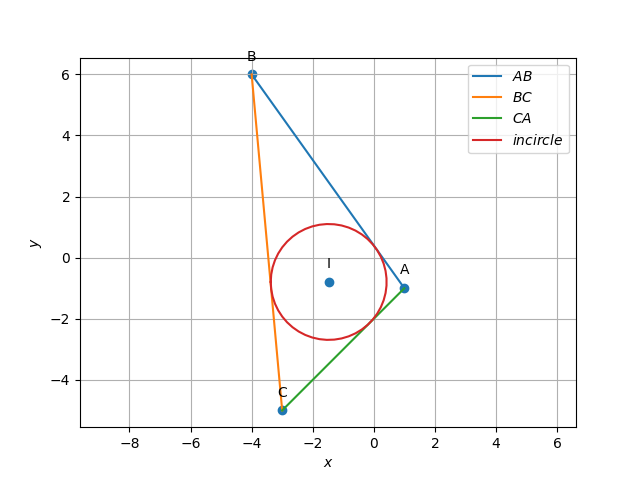
\includegraphics[width=\columnwidth]{solutions/1/5/7/figs/Diagram.png}
	\caption{Triangle with the incircle generated using python}
	\label{fig:Incircle}
\end{figure}

	The equation of the incircle is given as :

	\begin{align}
			\norm{\vec{x}-\vec{I}}^2 = r^2
	\end{align}

	\item Find the intersection $\vec{G}$ of $BE$ and $CF$.
 \\
\solution 
From 
	\eqref{eq:median-be}
	and
	\eqref{eq:median-cf},
the equations of $BE$ 
and 
$CF$
are, respectively,
\begin{align}
\myvec{3 & 1} \vec{x} &= \myvec{-6}
\label{eq:1.2.3,8}
\\
\myvec{ 5&-1} \vec{x} &= \myvec{-10}
\label{eq:1.2.3,9}
\end{align}
From \eqref{eq:1.2.3,8} and \eqref{eq:1.2.3,9} the augmented matrix is
\begin{align}
    \label{eq:matrowoperations}
    \myvec{
    3 & 1 & -6
    \\
    5 & -1 & -10
    }
     \xleftrightarrow[]{R_1 \leftarrow R_1+R_2}
    \myvec{
    8 & 0 & -16
    \\
    5 & -1 & -10 
    }
    \\
     \xleftrightarrow[]{R_1\leftarrow R_1/8}
    \myvec{
    1 & 0 & -2
    \\
    5 & -1 & -10 
    }
     \xleftrightarrow[]{R_2\leftarrow R_2-5R_1}
    \myvec{
    1 & 0 & -2
    \\
    0 & -1 & 0
    }
    \\
     \xleftrightarrow[]{R_2\leftarrow -R_2}
    \myvec{
    1 & 0 & -2
    \\
    0 & 1 & 0
    }
\end{align} 
using Gauss elimination.  Therefore, 
\begin{align}
\vec{G} = \myvec{-2 \\ 0}
	\label{eq:median-g}
\end{align}

	\item Verify that 
		\begin{align}
			\frac{BG}{GE} = 
			\frac{CG}{GF} =
			\frac{AG}{GD} =2 
		\end{align}
		\\	\solution 
\begin{enumerate}
\item From 
	\eqref{eq:median-e}
	and
	\eqref{eq:median-g},
\begin{align}
		\label{eq:tri-pts/4} \vec{G}-\vec{B} &= \myvec{2 \\ -6},\, 
 \vec{E}-\vec{G} = \myvec{1 \\ -3} \\
	\implies \vec{G}-\vec{B} &= 2 \brak{ \vec{E}-\vec{G} }
	\\
	\text{or, }		\label{eq:tri-pts/8}\frac{BG}{GE} &=  2  
\end{align}		
\item Calculating the ratio of $GF$ and $CG$,
\begin{align}
		\label{eq:tri-pts/9} \vec{F}-\vec{G} &= \myvec{\frac{1}{2} \\ \frac{5}{2}} \\
		\label{eq:tri-pts/10} \vec{G}-\vec{C} &= \myvec{1 \\ 5} \\
		\label{eq:tri-pts/11} \norm{\vec{F}-\vec{G}} &= \sqrt{\brak{\frac{1}{2}}^{2} + \brak{\frac{5}{2}}^{2}} &= \frac{\sqrt{26}}{2} \\  
		\label{eq:tri-pts/12} \norm{\vec{G}-\vec{C}} &= \sqrt{1^2 + 5^2} &= \sqrt{26} \\
		\label{eq:tri-pts/13}\frac{CG}{GF} &= \frac{\norm{\vec{G}-\vec{C}}}{\norm{\vec{F}-\vec{G}}} &= \frac{\sqrt{26}}{\frac{\sqrt{26}}{2}} &= 2		
\end{align}
\item Calculating the ratio of $AG$ and $GD$,
\begin{align}
		\label{eq:tri-pts/14} \vec{G}-\vec{A} &= \myvec{-3 \\ 1} \\
		\label{eq:tri-pts/15} \vec{D}-\vec{G} &= \myvec{\frac{-3}{2} \\ \frac{1}{2}} \\
		\label{eq:tri-pts/16} \norm{\vec{G}-\vec{A}} &= \sqrt{\brak{-3}^{2}+1^2} &= \sqrt{10} \\
		\label{eq:tri-pts/17} \norm{\vec{D}-\vec{G}} &= \sqrt{\brak{\frac{-3}{2}}^{2}+\brak{\frac{1}{2}}^{2}} &= \frac{\sqrt{10}}{2} \\
		\label{eq:tri-pts/18}\frac{AG}{GD} &= \frac{\norm{\vec{G}-\vec{A}}}{\norm{\vec{D}-\vec{G}}} &= \frac{\sqrt{10}}{\frac{\sqrt{10}}{2}} &= 2 
\end{align}
\end{enumerate}
From \eqref{eq:tri-pts/8}, \eqref{eq:tri-pts/13}, \eqref{eq:tri-pts/18}
\begin{align}
		\frac{BG}{GE} = 
		\frac{CG}{GF} =
		\frac{AG}{GD} = 2
\end{align}
Hence verified.

	\item Show that $\vec{A}, \vec{G}$ and $\vec{D}$ are collinear.
	\\
		\solution 
Points $\vec{A},\vec{D},\vec{G}$ are defined to be collinear if 
\begin{align}
    \text{rank}\myvec{
    1 & 1 & 1\\
    \vec{A} & \vec{D} & \vec{G} \\
    } = 2 
    \label{eq:mat_row_operations}
    \\
\implies    
    \myvec{
    1 & 1 & 1
    \\
    1 & -\frac{7}{2} & -2
    \\
    -1 & \frac{1}{2} & 0
    }
     \xleftrightarrow[]{R_3 \leftarrow R_3+R_2}
    \myvec{
    1 & 1 & 1
    \\
    1 & -\frac{7}{2} & -2
    \\
    0 & -3 & -2 
    }
    \\
     \xleftrightarrow[]{R_2\leftarrow R_2-R_1}
    \myvec{
    1 & 1 & 1
    \\
    0 & -\frac{9}{2} & -3
    \\
    0 & -3 & -2 
    }
     \xleftrightarrow[]{R_3\leftarrow R_3-\frac{2}{3}R_2}
    \myvec{
    1 & 1 & 1
    \\
    0 & -\frac{9}{2} & -3
    \\
    0 & 0 & 0
    }
\end{align}
Thus, the matrix 
    \eqref{eq:mat_row_operations}
    has rank 2 and the points are collinear.

	\item Verify that 
		\begin{align}
			\vec{G}=\frac{\vec{A}+\vec{B}+\vec{C}}{3}
		\end{align}
			$\vec{G}$ is known as the {\em centroid} of $\triangle ABC$.
   \\
		\solution
\begin{equation}
\begin{split}
\label{eq:centroid}
    \vec{G}&= \frac{\myvec{1\\-1}+\myvec{-4\\6}+\myvec{-3\\-5}}{3}\\    
     &= \myvec{-2\\0}
\end{split}
\end{equation}

 




	\item Verify that 
		\begin{align}
\vec{A}-\vec{F}=\vec{E}-\vec{D}
		\end{align}
		The quadrilateral $AFDE$ is defined to be a parallelogram.\\
  		\\ \solution 
\begin{align}
    \vec{A}-\vec{F}&=\myvec{1\\-1}-\myvec{\frac{-3}{2}\\\frac{5}{2}}
    =\myvec{\frac{5}{2}\\\frac{-7}{2}}
    \\
    \vec{E}-\vec{D}&=\myvec{-1\\-3}-\myvec{\frac{-7}{2}\\\frac{1}{2}}
    =\myvec{\frac{5}{2}\\\frac{-7}{2}}
    \\
	\implies	\vec{A}-\vec{F} &= \vec{E}-\vec{D}
\end{align}
See \figref{fig:Triangle}, 
\begin{figure}
\centering
\includegraphics[width=\columnwidth]{solutions/1/2/7/figs/figure1.png}
\caption{$AFDE$ form a parallelogram in triangle ABC}
\label{fig:Triangle}
\end{figure}






















  
\end{enumerate}
